% =====================================================================
%  INMIC 2026 -- Paper ID 159 -- conference talk (10-12 min, 14 slides)
%  CSR-MMDiff: Clear-Sky-Residual Multimodal Diffusion for Probabilistic
%  PV Forecasting
%
%  Build:  pdflatex INMIC2026_Paper159_Slides   (run twice)
%  Speaker notes: change the \setbeameroption line below to
%     \setbeameroption{show notes on second screen=right}
%  or  \setbeameroption{show only notes}
% =====================================================================
\documentclass[aspectratio=169,11pt]{beamer}
\usetheme{INMIC}
\usepackage{amsmath,amssymb}
\setbeameroption{hide notes}
\graphicspath{{figures/}}

\renewcommand{\inmicfootertext}{CSR-MMDiff \textperiodcentered{} INMIC 2026 \textperiodcentered{} Paper 159}

\title{CSR-MMDiff: Clear-Sky-Residual Multimodal Diffusion for Probabilistic PV Forecasting}
\subtitle{INMIC 2026 \textperiodcentered{} Paper ID 159}
\author{Muhammad Umer, Haseeb Ullah, Jameel Ahmad, Syed Baqar Hussain, Abdul Hameed}
\institute{Department of Computer Science, SST, University of Management and Technology, Lahore}
\date{28th International Multitopic Conference \textperiodcentered{} UET Lahore \textperiodcentered{} 25--26 November 2026}

\begin{document}

% ---------------------------------------------------------------------
{\setbeamertemplate{footline}{}
\begin{frame}
\titlepage
\note{Good [morning/afternoon]. I am [presenter name] from the School of Systems and Technology at UMT Lahore. Our paper, CSR-MMDiff, is about probabilistic forecasting of photovoltaic power a few minutes ahead, using sky images and a diffusion model. The one-line idea: instead of asking the diffusion model to generate the whole future, we let it generate only the deviation from a simple physical forecast.}
\end{frame}}

% ---------------------------------------------------------------------
\begin{frame}{Why another diffusion model for PV forecasting?}{Motivation}
\begin{columns}[T]
\begin{column}{0.48\textwidth}
\begin{card}{Ramps need distributions}\small
A passing cloud can halve a PV plant's output within a minute. Grid operators need the full distribution of future output, not one number. Sky cameras show the clouds coming.
\end{card}
\end{column}
\begin{column}{0.48\textwidth}
\begin{card}{Our earlier models fell short}\small
\textbf{B1} (15-step DDIM): 77.9\% coverage, median biased low and worse than persistence, frames blurred within minutes.\\
\textbf{B2} (10-step DDIM): 100$\times$ faster than DDPM, but coverage fell from 87.5\% to 64.8\%.
\end{card}
\end{column}
\end{columns}
\vspace{2mm}
\begin{callout}
Both models spend capacity re-generating what is already known: the daily PV cycle and the static sky.
\end{callout}
\note{Ultra-short-term PV forecasting matters because clouds cause ramps: output can halve within a minute, and numerical weather prediction cannot see that. Operators therefore need a distribution of future output. Our two earlier models had clear problems. B1 had intervals covering only 77.9 percent, a median biased low and worse than persistence, and blurry frames. B2 showed that 10-step DDIM is 100 times faster than DDPM but loses calibration. Our diagnosis: both models waste capacity regenerating things we already know.}
\end{frame}

% ---------------------------------------------------------------------
\begin{darkframe}
\begin{frame}{Diffuse only the deviation from a physical prior}{Key idea}
\begin{columns}[T]
\begin{column}{0.48\textwidth}
\begin{darkcard}{PV power}
\[\color{inmicPaper} x^P_{0,k}=\frac{P_{t+k}-\hat P^{\mathrm{SPM}}_{t+k}}{s_P}\]
\small Residual from \textbf{clear-sky smart persistence}: the clear-sky index $k_t=P_t/P^{\mathrm{clr}}_t$ is held constant; clear-sky power from the pvlib Ineichen model.
\end{darkcard}
\end{column}
\begin{column}{0.48\textwidth}
\begin{darkcard}{Sky images}
\[\color{inmicPaper} \mathbf x^I_{0,k}=\frac{\mathbf I_{t+k}-\mathbf I_t}{s_I}\]
\small Residual from the \textbf{last observed frame}: sun position, lens rings and static sky need not be re-generated.
\end{darkcard}
\end{column}
\end{columns}
\vspace{3mm}
A zero residual \textbf{equals persistence}, so the network only models cloud-induced deviations.
\note{This is the central idea. Instead of diffusing raw future PV power, we diffuse its residual from clear-sky smart persistence, which keeps the current clear-sky index constant and multiplies it by the clear-sky power from the pvlib Ineichen model. For images we diffuse the difference from the last observed frame. If the model outputs zero, it reproduces persistence exactly, so the network only has to learn how clouds make the future differ from that baseline.}
\end{frame}
\end{darkframe}

% ---------------------------------------------------------------------
\begin{frame}{Coupled U-Net with cloud-aware cross-modal attention}{Model}
\centering
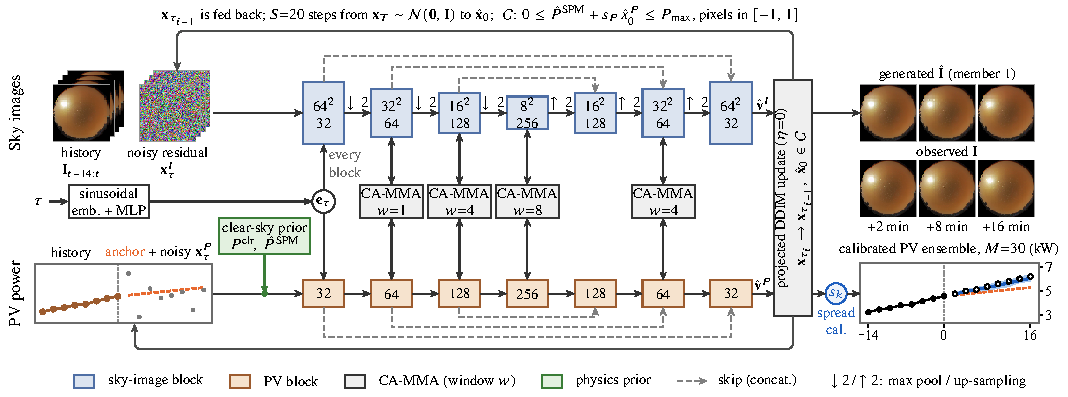
\includegraphics[width=\textwidth,height=0.52\textheight,keepaspectratio]{fig_arch.pdf}
\vspace{2mm}
\begin{columns}[T]
\begin{column}{0.31\textwidth}\small\textbf{5.1\,M parameters}: two four-level branches (32--256 channels).\end{column}
\begin{column}{0.31\textwidth}\small\textbf{CA-MMA}: learned spatial pooling keeps where clouds sit relative to the sun.\end{column}
\begin{column}{0.31\textwidth}\small\textbf{Conditioning}: clear-sky power known ahead, plus modality flags.\end{column}
\end{columns}
\note{The denoiser is a coupled U-Net with an image branch and a PV branch, 5.1 million parameters. Earlier models pooled each image frame into one token by averaging, which throws away where clouds are relative to the sun. Our cloud-aware attention learns four spatial attention maps instead, initialised to average pooling. The PV branch is conditioned on the clear-sky power, known in advance, and on flags saying which modality is available.}
\end{frame}

% ---------------------------------------------------------------------
\begin{frame}{Projected DDIM sampling with lead-wise spread calibration}{Training and sampling}
\begin{columns}[T]
\begin{column}{0.32\textwidth}
\begin{navycard}{Training}\small
v-prediction on a cosine schedule ($T=1000$), Min-SNR loss weighting; images-only and PV-only inputs in 15\% of windows each.
\end{navycard}
\end{column}
\begin{column}{0.32\textwidth}
\begin{navycard}{Projected DDIM}\small
20 deterministic steps. Each clean estimate is projected so that $0\le$ PV $\le 30$\,kW and pixels stay in $[-1,1]$.
\end{navycard}
\end{column}
\begin{column}{0.32\textwidth}
\begin{goldcard}{Spread calibration}\small
Members scaled around the median by $s_k\in[0.5,3]$ per lead, fitted on 1{,}536 validation windows. The median is unchanged.
\end{goldcard}
\end{column}
\end{columns}
\note{Training uses v-prediction on a cosine noise schedule with Min-SNR weighting; some training windows hide one modality. At sampling time we run 20 DDIM steps and project the clean estimate onto physically feasible values at every step. Finally, a calibration scales each member's distance from the ensemble median by one factor per lead time, fitted on validation days only. Every point metric stays the same.}
\end{frame}

% ---------------------------------------------------------------------
\begin{frame}{SKIPP'D benchmark, same test windows as B1}{Experimental setup}
\small
\renewcommand{\arraystretch}{1.25}
\begin{tabular}{@{}p{0.2\textwidth}p{0.74\textwidth}@{}}
\headrow \thc{Item} & \thc{Setting}\\
Data & $64\times64$ sky images + power of a 30\,kW array at Stanford; 2-min cadence; leads 2--16\,min\\
\rowcolor{inmicRow} Split & Train / validation by calendar day: 447 / 50 days\\
Test & 1{,}340 windows on 20 clear, partly cloudy and overcast days\\
\rowcolor{inmicRow} Cloudy subset & 5 most variable days, 1{,}199 windows (selected using observed PV)\\
Baselines & Smart persistence, persistence ensemble (PeEn), B1 and its two-stage pipeline, B2, B3\\
\rowcolor{inmicRow} Compute & 2 $\times$ RTX 3080, 7.9\,h training; 30 members per forecast\\
\end{tabular}
\note{We use SKIPP'D from Stanford. Training and validation are split by calendar day. The test set is exactly the 1,340 windows on which B1 was evaluated, so that comparison is like-for-like. The cloudy subset mirrors PV-MM-Diffusion's protocol but is selected using the observed power, so it is not an operational setting.}
\end{frame}

% ---------------------------------------------------------------------
\begin{frame}{22.9\% lower CRPS than our previous model}{Main result \textperiodcentered{} 1,340 test windows}
\begin{columns}[T]
\begin{column}{0.66\textwidth}
\small\renewcommand{\arraystretch}{1.25}
\begin{tabular}{@{}lrrrr@{}}
\headrow \thc{Method} & \thc{CRPS} & \thc{WS$_{90}$} & \thc{Cov.} & \thc{MAE}\\
Smart persistence & 1.322 & -- & -- & 1.322\\
\rowcolor{inmicRow} PeEn & 1.177 & 18.92 & 76.9\% & 1.315\\
B1 joint DDIM & 1.222 & 10.50 & 77.9\% & 1.684\\
\rowcolor{inmicRow} Ours, uncalibrated & 0.995 & 12.33 & 57.4\% & 1.243\\
\hlrow \textbf{CSR-MMDiff} & \textbf{0.943} & \textbf{9.15} & \textbf{83.2\%} & \textbf{1.243}\\
\end{tabular}\\[2mm]
{\scriptsize\color{inmicMuted} kW; WS$_{90}$: Winkler score of the 90\% interval; Cov.: its coverage (nominal 90\%).}
\end{column}
\begin{column}{0.3\textwidth}
\begin{bignum}\bigtxt{28.7\%}\\\small CRPS skill over smart persistence\end{bignum}
\begin{bignum}\bigtxt{$-$6.0\%}\\\small median MAE vs.\ persistence\end{bignum}
\end{column}
\end{columns}
\note{On identical windows, CSR-MMDiff reaches a CRPS of 0.943 kilowatts: 22.9 percent below B1 and 28.7 percent below smart persistence. The Winkler score drops from 10.5 to 9.15, and the median beats persistence as a point forecast. The uncalibrated row matters: the CRPS is already 0.995 before calibration, but coverage is only 57 percent.}
\end{frame}

% ---------------------------------------------------------------------
\begin{frame}{Better at every lead, with sharper and steadier intervals}{By lead time}
\centering
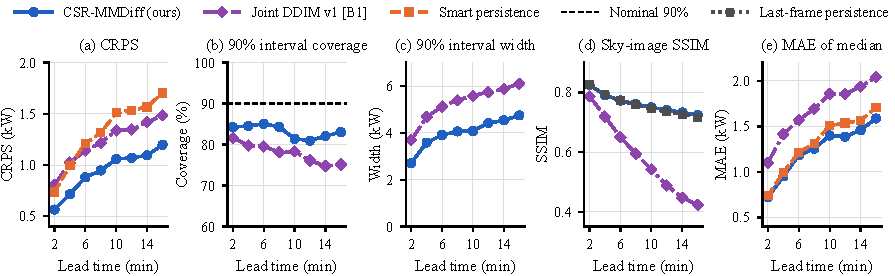
\includegraphics[width=\textwidth,height=0.5\textheight,keepaspectratio]{fig_lead.pdf}
\vspace{2mm}
\begin{columns}[T]
\begin{column}{0.31\textwidth}\small\textbf{Skill} rises from 23\% at +2\,min to about 30\% beyond +10\,min.\end{column}
\begin{column}{0.31\textwidth}\small\textbf{Coverage} stays at 81--85\% per lead; B1 fell from 81.6\% to 75.1\%.\end{column}
\begin{column}{0.31\textwidth}\small\textbf{Width} 2.7--4.7\,kW vs.\ 3.7--6.1\,kW for B1.\end{column}
\end{columns}
\note{The gain holds at every lead: 23 percent skill at 2 minutes, where B1 was worse than persistence, rising to about 30 percent beyond 10 minutes. Coverage stays between 81 and 85 percent while B1 decayed to 75 percent, and our intervals are narrower at the same time.}
\end{frame}

% ---------------------------------------------------------------------
\begin{frame}{The model brings the CRPS gain; calibration fixes coverage}{Calibration}
\begin{columns}[T]
\begin{column}{0.32\textwidth}
\begin{card}{}{\Large\bfseries\color{inmicNavy}57.4\%\,$\to$\,83.2\%}\\[1mm]\small 90\% coverage before and after calibration\end{card}
\end{column}
\begin{column}{0.32\textwidth}
\begin{card}{}{\Large\bfseries\color{inmicNavy}$\approx 2\times$}\\[1mm]\small spread factors $s_k=1.95$--$2.25$, nearly constant over leads\end{card}
\end{column}
\begin{column}{0.32\textwidth}
\begin{card}{}{\Large\bfseries\color{inmicNavy}$-$18.6\%}\\[1mm]\small CRPS vs.\ B1 \textbf{before} calibration ($-$15.5\% vs.\ PeEn)\end{card}
\end{column}
\end{columns}
\vspace{2mm}
\begin{callout}
The raw ensemble is sharp but under-dispersed. Calibration lowers the Winkler score by 25.8\% and CRPS by a further 5.2\%. B1 was not recalibrated the same way.
\end{callout}
\note{How much is calibration? Most of the coverage, but not most of the CRPS. The raw ensemble covers only 57 percent; spread factors are about two at every lead. After calibration, coverage is 83 percent. But the CRPS before calibration is already 18.6 percent below B1 and 15.5 percent below the persistence ensemble. Caveat: B1 was not recalibrated the same way.}
\end{frame}

% ---------------------------------------------------------------------
\begin{frame}{Frames stay anchored to the scene instead of fading to haze}{Generated sky images}
\centering
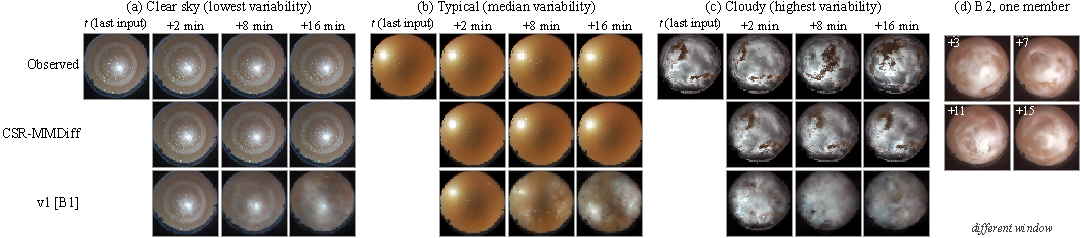
\includegraphics[width=\textwidth,height=0.45\textheight,keepaspectratio]{fig_images.pdf}
\vspace{2mm}
\begin{columns}[T]
\begin{column}{0.31\textwidth}\small\textbf{SSIM at +16\,min:} 0.724 vs.\ 0.423 for B1.\end{column}
\begin{column}{0.31\textwidth}\small\textbf{VGG-CS:} 0.959 vs.\ 0.862 for B1.\end{column}
\begin{column}{0.31\textwidth}\small\textbf{But:} SSIM stays within 0.01 of last-frame persistence; clouds barely move.\end{column}
\end{columns}
\note{Because images are generated as a residual from the last frame, the sun, lens rings and cloud layout persist, whereas B1's frames dissolve into haze. But our SSIM stays within 0.01 of repeating the last frame and the clouds barely move: the image branch has learned little advection, and the PV gain comes from the residual formulation.}
\end{frame}

% ---------------------------------------------------------------------
\begin{frame}{Clear days are tracked; fast ramps still arrive late}{Whole-day forecasts}
\begin{columns}[c]
\begin{column}{0.42\textwidth}
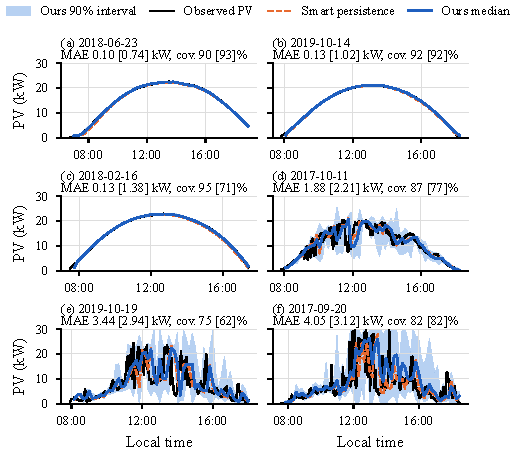
\includegraphics[width=\linewidth,height=0.66\textheight,keepaspectratio]{fig_days.pdf}
\end{column}
\begin{column}{0.55\textwidth}
\begin{navycard}{Clear days}\small
+16\,min MAE 0.10--0.13\,kW vs.\ 0.74--1.38\,kW for B1, without B1's spurious afternoon dips.
\end{navycard}
\begin{goldcard}{Two most variable days}\small
The median lags ramps like persistence: +16\,min MAE 3.44 vs.\ 2.94 and 4.05 vs.\ 3.12\,kW, \textbf{worse than B1}, although coverage is higher (75\% vs.\ 62\%).
\end{goldcard}
\end{column}
\end{columns}
\note{On clear days the median follows the observation almost exactly. On the two most variable days, however, the median reproduces ramps late, like persistence, and its 16-minute error is worse than B1's, even though its interval covers more observations. Since ramps motivate this work, this is the main weakness of the current model.}
\end{frame}

% ---------------------------------------------------------------------
\begin{frame}{Close to the full-size model's skill at a fraction of the cost}{Cost and context}
\begin{columns}[T]
\begin{column}{0.48\textwidth}
{\small\bfseries\color{inmicNavy} DDIM steps (validation)}\\[1mm]
\small\renewcommand{\arraystretch}{1.2}
\begin{tabular}{@{}lrr@{}}
\headrow \thc{Steps} & \thc{CRPS (kW)} & \thc{ms/member}\\
5 & 0.653 & 13\\
\rowcolor{inmicRow} 10 & 0.640 & 24\\
\hlrow \textbf{20 (used)} & \textbf{0.617} & \textbf{51}\\
\rowcolor{inmicRow} 50 & 0.613 & 134\\
\end{tabular}\\[1mm]
{\scriptsize\color{inmicMuted}$\eta=0$ beats $\eta=0.5$ and 1; sky-image guidance hurts.}
\end{column}
\begin{column}{0.48\textwidth}
{\small\bfseries\color{inmicNavy} Cloudy-day protocol (skill vs.\ own SPM)}\\[1mm]
\small\renewcommand{\arraystretch}{1.2}
\begin{tabular}{@{}lr@{}}
\headrow \thc{Method} & \thc{Skill}\\
SkyGPT$\to$U-Net & 12.5\%\\
\rowcolor{inmicRow} PV-MM-Diffusion (8 GPUs) & 28.3\%\\
\hlrow \textbf{CSR-MMDiff (2 GPUs)} & \textbf{25.4\%}\\
\end{tabular}\\[1mm]
{\scriptsize\color{inmicMuted}Different test days and SPM per study: relative skill only.}
\end{column}
\end{columns}
\note{Twenty DDIM steps get almost all of the benefit of fifty at less than half the cost; deterministic sampling works best. Test sampling takes 54 milliseconds per member. On the cloudy subset we reach 25.4 percent skill versus 28.3 percent reported for PV-MM-Diffusion with eight GPUs; protocols differ, so only relative skill is comparable.}
\end{frame}

% ---------------------------------------------------------------------
\begin{frame}{What the evidence does not yet show}{Limitations and next steps}
\begin{columns}[T]
\begin{column}{0.48\textwidth}
\begin{card}{Limitations}\small
\begin{itemize}
\item Coverage 6.8 points below nominal; 13.9 below on cloudy windows
\item Median lags ramps; little cloud advection learned
\item One site, 20 test days, one training run, no confidence intervals
\item Residual target, CA-MMA and projection not ablated one by one
\end{itemize}
\end{card}
\end{column}
\begin{column}{0.48\textwidth}
\begin{card}{Next steps}\small
\begin{itemize}
\item Weather-regime-conditional or conformal calibration
\item Longer image context to learn cloud motion
\item Component ablations and repeated runs with bootstrap intervals
\item Non-diffusion baselines: quantile regression, MC dropout
\end{itemize}
\end{card}
\end{column}
\end{columns}
\note{Coverage is still below nominal, much more on cloudy windows. The median lags on ramp days and the image branch learns little advection. One site, twenty test days, one run without confidence intervals, and several components introduced together. Next: regime-conditional or conformal calibration, longer image history, ablations with repeated runs, and non-diffusion baselines.}
\end{frame}

% ---------------------------------------------------------------------
\begin{darkframe}
\begin{frame}{Conclusion}
\vspace{1mm}
{\large\bfseries Putting a physical forecast inside the diffusion target makes a small model a probabilistic correction of persistence.\par}
\vspace{3mm}
{\small\color{inmicOnDark} CRPS 0.943\,kW ($-$22.9\% vs.\ B1, 28.7\% skill over smart persistence) \textperiodcentered{} 83.2\% coverage with narrower intervals \textperiodcentered{} median beats persistence \textperiodcentered{} 54\,ms per member. Open problems: cloudy-day coverage and ramp timing.\par}
\vfill
{\Large\bfseries\color{inmicGold} Thank you \textperiodcentered{} Questions?\par}
{\scriptsize\color{inmicOnDark} f2023266912@umt.edu.pk \textperiodcentered{} jameel.ahmad@umt.edu.pk\par}
\vspace{2mm}
\note{By diffusing sky-image and PV residuals with respect to a clear-sky persistence prior, a 5-million-parameter model lowers the CRPS of our previous model by 23 percent, reaches 83 percent coverage with narrower intervals, beats persistence as a point forecaster, and samples in 54 milliseconds per member. Open problems: coverage on cloudy days and ramp timing. Thank you.}
\end{frame}
\end{darkframe}

\end{document}
